\documentclass[review]{elsarticle}
\usepackage[spanish]{babel}
\usepackage{graphicx}
\usepackage{subfig}
\usepackage{lineno,hyperref}
\usepackage{natbib}
\setcitestyle{numbers,sort&compress}
\usepackage{float}
\usepackage{footmisc}
\usepackage{adjustbox}
\usepackage{tikz}
\usepackage{listing}
\usepackage{pythonhighlight}
\usepackage{rotating}
\usepackage{array,booktabs,makecell}
\usepackage{amssymb}
\modulolinenumbers[5]

%\journal{Journal of \LaTeX\ Templates}


\newenvironment{abstracts}
 {\global\setbox\absbox=\vbox\bgroup
    \hsize=\textwidth
    \linespread{1}\selectfont}
 {\vspace{-\bigskipamount}\egroup}
\renewenvironment{abstract}[1][]
 {\if\relax\detokenize{#1}\relax\else\selectlanguage{#1}\fi
  \noindent\textbf{\abstractname}\par\medskip\noindent\ignorespaces}
 {\par\bigskip}
 
 
\let\today\relax
\makeatletter
\def\ps@pprintTitle{%
    \let\@oddhead\@empty
    \let\@evenhead\@empty
    \def\@oddfoot{\footnotesize\itshape
         {} \hfill\today}%
    \let\@evenfoot\@oddfoot
    }
\makeatother
%%%%%%%%%%%%%%%%%%%%%%%
%% Elsevier bibliography styles
%%%%%%%%%%%%%%%%%%%%%%%
%% To change the style, put a % in front of the second line of the current style and
%% remove the % from the second line of the style you would like to use.
%%%%%%%%%%%%%%%%%%%%%%%

%% Numbered
%\bibliographystyle{model1-num-names}

%% Numbered without titles
%\bibliographystyle{model1a-num-names}

%% Harvard
%\bibliographystyle{model2-names.bst}\biboptions{authoryear}

%% Vancouver numbered
%\usepackage{numcompress}\bibliographystyle{model3-num-names}

%% Vancouver name/year
%\usepackage{numcompress}\bibliographystyle{model4-names}\biboptions{authoryear}

%% APA style
%\bibliographystyle{model5-names}\biboptions{authoryear}

%% AMA style
%\usepackage{numcompress}\bibliographystyle{model6-num-names}

%% `Elsevier LaTeX' style
\bibliographystyle{mighelnat}
%%%%%%%%%%%%%%%%%%%%%%%

\begin{document}

\begin{frontmatter}

\title{Inventarios forestales a través del procesamiento de imágenes}


\author{José Angel Ramírez Cantú}
\author{Satu Elisa Schaeffer}

\address{San Nicolás de los Garza, Nuevo León, México}

\begin{abstracts}
\begin{abstract}[spanish]
El impacto de la visión computacional en distintas áreas tiene un impacto positivo dando como resultado el poder resolver problemas de sectores diferentes a los de la tecnología. Es por eso que este trabajo propone utilizar la visión computacional en conjunto con el aprendizaje máquina para automatizar la clasificación de especies arbóreas y generación de inventarios forestales con el fin de reemplazar a las técnicas tradicionales que se utilizan en el sector forestal.
\end{abstract}

\textit{Palabras clave: } Procesamiento de imágenes, Aprendizaje máquina, Inteligencia artificial, Visión Computacional, Inventarios forestales.
\vspace*{0.5cm}
\end{abstracts}


\end{frontmatter}

\section{Introducción}

Este trabajo explica el funcionamiento de la solución propuesta para generar inventarios forestales utilizando el procesamiento de imágenes para la generación de inventarios forestales. Dicha solución consta de seis fases en las que se las que hace uso de muestras generadas a partir del recorrido de un dron en la zona del Cilantrillo y Trinidad (véanse las figuras \ref{Zona-cilantrillo} y \ref{Zona-trinidad} de la página \pageref{Zona-trinidad}). 

%%Duda #1, puedo referirme a las figuras de la misma página en una misma frase?

Aunque ya existen algunas software de computadora que ya tienen la facultad de poder detectar objetos, hay pocas soluciones que vayan totalmente enfocadas a generar inventarios forestales utilizando haciendo uso de tecnologías innovadoras que necesiten la menor interacción posible con el usuario que necesite generar un inventario forestal.
\clearpage

\begin{figure}[h!]
  \centering
\begin{tabular}{@{}ccc@{}}
\subfloat[Estatal]{\includegraphics[width=0.30\textwidth]{Lejos_C}} & 
\subfloat[Municipal]{\includegraphics[width=0.30\textwidth]{Medio_C}} &
\subfloat[Local]{\includegraphics[width=0.30\textwidth]{Cerca_C}}
  \end{tabular}
  \caption[Mapa de Cilantrillo]{El Cilantrillo, Montemorelos, Nuevo León (25.3523418, -100.3463186).}
   \label{Zona-cilantrillo}
\end{figure}

\begin{figure}[h!]
  \centering
\begin{tabular}{@{}ccc@{}}
\subfloat[Estatal]{\includegraphics[width=0.30\textwidth]{Lejos_t}} & 
\subfloat[Municipal]{\includegraphics[width=0.30\textwidth]{Medio_t}} &
\subfloat[Local]{\includegraphics[width=0.30\textwidth]{Cerca_t}}
  \end{tabular}
  \caption[Mapa de Trinidad.]{La Trinidad, Santiago, Nuevo León (25.225939, -100.1431609).}
  \label{Zona-trinidad}
\end{figure}

El objetivo de este trabajo es demostrar que la solución propuesta puede reducir tiempos a la hora de procesar las muestras recolectadas por el recorrido de un dron e identificar por sí misma, cada especie presente en las muestras recolectadas haciendo uso del procesamiento de imágenes. Otro de los objetivos es extraer la información de cada especie con el fin de generar un modelo a partir de la información recolectada en las especies de arboles definidas.\\

El artículo está divido en seis secciones, la sección 2 define los conceptos clave para el entendimiento del artículo, la sección 3 se presenta los artículos relacionados al presente trabajo y su diferencia, la sección 4 detalla la solución propuesta así como su metodología, la sección 5 se expone los resultados que apoyan a la hipótesis planteada  y los experimentos que permiten reafirmar la hipótesis inicial, finalmente la sección 6 presenta las conclusiones del artículo desarrollado y la contribución del presente artículo.

\section{Antecedentes}
La \emph{inteligencia artificial}\footnote{Ciencia encargada de desarrollar algoritmos capaces de imitar capacidades humanas} es una de las tecnologías que más ha acaparado la atención no sólo de las personas, sino también de las compañías que la utilizan con distintos fines, tanto cotidianos como industriales. Sin embargo, el porque de utilizarlas no sólo es con el fin de reemplazar las capacidades de un ser humano, sino que buscan facilitar las acciones con las que interactúa cada persona. En el caso del artículo se detalla como es que se busca utilizar la técnica de  \emph{procesamiento de imágenes}\footnote{Su función es capturar y procesar por medio de imágenes las información más relevante} para trabajar en conjunto con el \emph{aprendizaje máquina}\footnote{Campo de la inteligencia artificial que desarrolla algoritmos capaces de aprender por medio de información.} en el análisis de zonas forestales haciendo uso de \emph{clasificación de imágenes}\footnote{Es una técnica del aprendizaje máquina que consiste en identificar un objeto por medio de propiedades o características propias de un elemento.}.\\

El procesamiento de imágenes puede enfocarse en la búsqueda de un elemento en particular, por lo que permitiría reducir el tiempo que se invierte en clasificar individualmente cada especie de árbol y podría, paralelamente, identificar cada especie presente  a lo largo de un sector forestal no centrándose únicamente en una sola especie. Cabe destacar que el procesamiento de imágenes no sería posible sin la intervención de la \emph{visión computacional}\footnote{Técnica de la inteligencia artificial que intenta emular la capacidad visual de los humanos.} la cual es la que permitiría el detectar automáticamente cada especie en la solución propuesta.\\

%duda 2, puedo citar a alguien en un footnote?
En el caso de los \emph{inventarios forestales}\footnote{ref... lo define como sistemas de recolección de características del área sobre el que se trabaja}, se va utilizar el procesamiento de imágenes para analizar las características de \textit{forma, color, bordes, textura} en las muestras, posteriormente el aprendizaje máquina tendrá que establecer en un modelo de información el análisis obtenido a partir de las características previamente mencionadas.

\subsection{Antecedentes históricos}
El procesamiento de imágenes surge en el año 1920 de los primeros intentos de transmisión de imágenes por medio de un cable transatlántico usando códigos telegráficos, permitiendo la codificación de una imagen en cinco niveles de gris para posteriormente, en 1929, el ya mencionado sistema de transmisión permitía codificar a quince niveles de gris, a su vez, este sistema redujo el tiempo de transmisión de imágenes a quince minutos (incluir cita).\\

El aprendizaje máquina surge a principios del año 1990 como un proceso para la extracción de información y modelos de predicción, esto último fue bastante utilizado por los sectores bancarios, que eran los que mayormente le sacaban un provecho a la hora de tomar decisiones (incluir cita).\\ 

La visión computacional llevaba bastante más tiempo que había sido desarrollada, pero no empleada; y es que en el año 1960 es cuando la inteligencia artificial apenas se estaba desarrollando y fue cuando se planteo el como es que una computadora iba a razonar como lo haría una persona. Los problemas recaen sobre factores de innovación y procesamiento de imágenes automático.

\subsection{Descriptores de características globales}
Existen dos tipos de características utilizados en el presente trabajo, las características globales que son las que pueden percibirse fácilmente (color, forma, textura) y las características locales, que cuantifican globalmente una imagen, estas últimas son necesarias son necesarias para determinar que descriptor de características es el mejor para describir los puntos de interés o cierta región de una imagen.
\clearpage

\subsubsection{Color}
La característica de clasificación de color hace uso del \emph{histograma de color}\footnote{Cantidad de pixeles en listas de rangos de colores presentes en una imagen.} y por medio de gráficas, determinar la intensidad de la distribución del valor de un \emph{pixel}\footnote{Es la unidad básica más pequeña de las imágenes.}.

\begin{figure}[h!]
  \centering
\begin{tabular}{@{}ccc@{}}
\subfloat[Muestra utilizada]{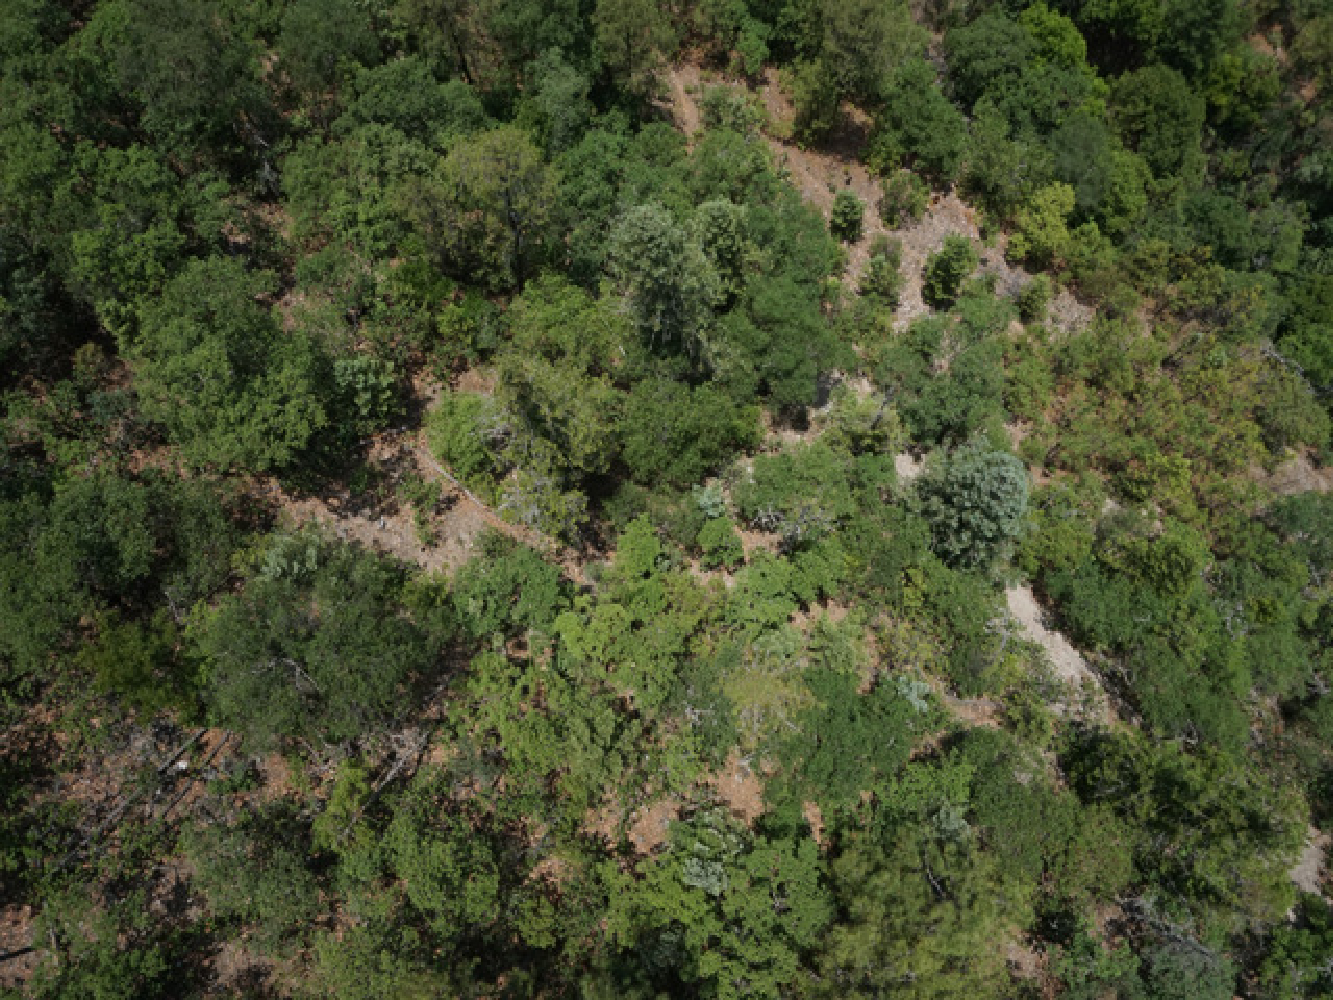
\includegraphics[width=0.45\textwidth]{DSC06100}} & 
\subfloat[Histograma generado]{\includegraphics[width=0.45\textwidth]{histograma-gen}} &
  \end{tabular}
  \caption[Histograma de color]{Histograma de color generado con las bibliotecas \texttt{matplotlib y OpenCV.}}
  \label{Histograma-generado}
\end{figure}

\subsubsection{Forma}
La característica de forma cuenta también con varias métricas, se hace énfasis en los \emph{momentos de una imagen}. Los momentos de una imagen son los pesos promedio de la intensidad de píxel sobre una imagen.

\begin{figure}[h!]
  \centering
    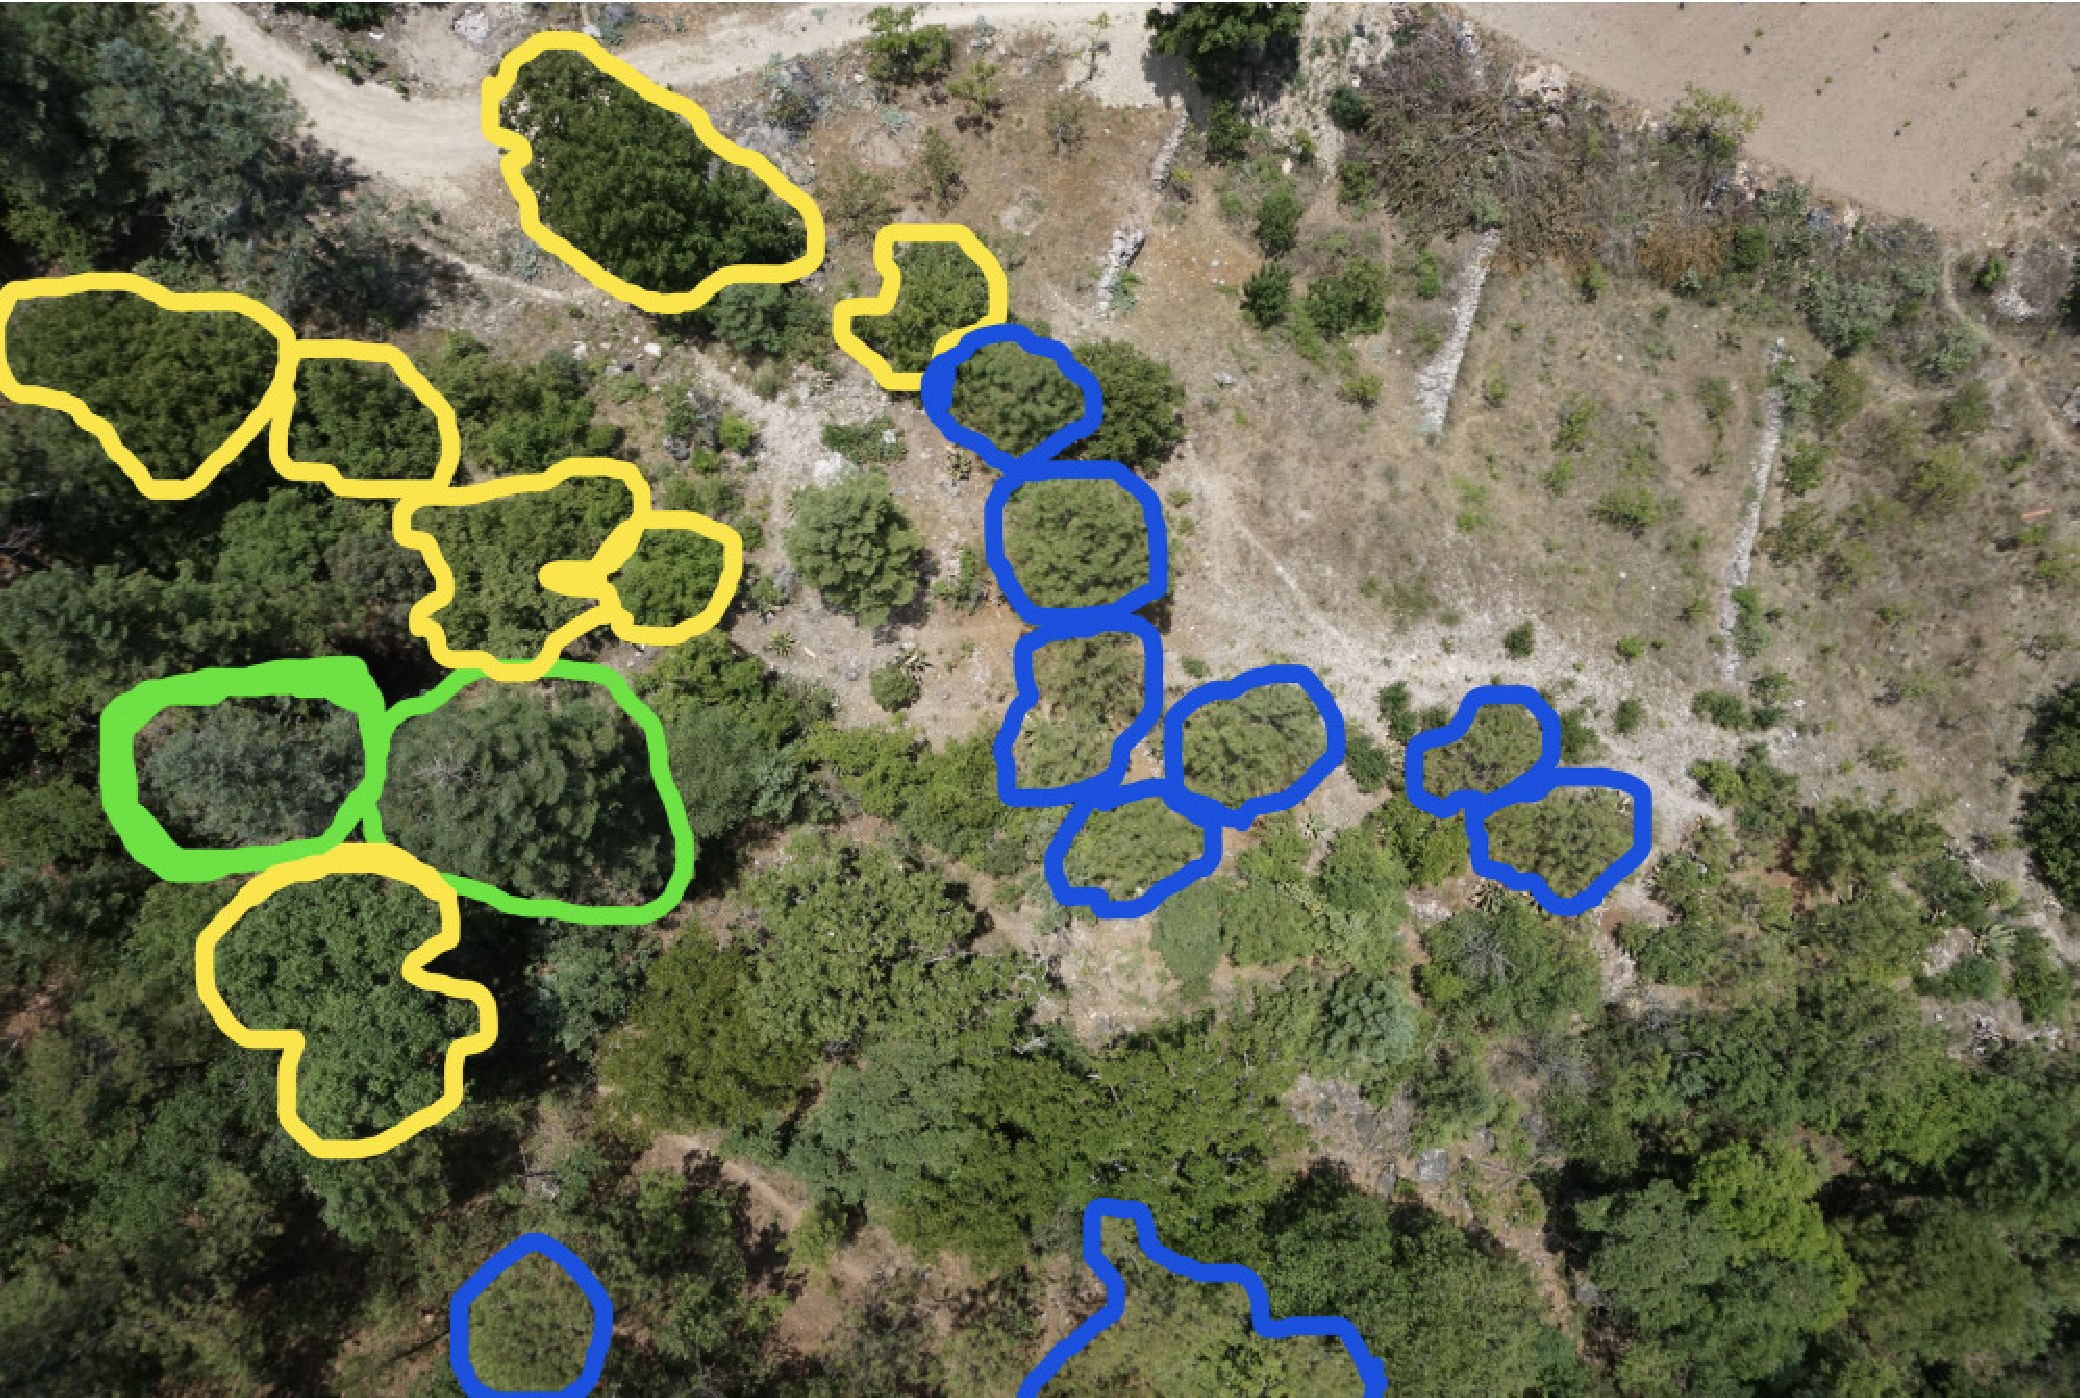
\includegraphics[width=0.45\textwidth]{Anotaciones-ex}
    \caption[Formas de cada especie arbórea.]{Formas de cada especie arbórea (verde: Abies, azúl: Pino, amarillo: Encino).}
\end{figure}

\clearpage

\subsubsection{Textura}
Esta característica tiene una gran relevancia dado que es de las más usadas al momento de identificar objetos en regiones de interés en fotografías aéreas, micrográficas y de satélite y en el presente trabajo, al identificar las muestras de los árboles. En este caso se emplea la métrica de \emph{textura de Haralick}.\\

Esta métrica o conjunto de descriptores estadísticos de textura realizada por (citar), se utiliza como parte de un conjunto de descriptores estadísticos de textura para determinar 14 descriptores de textura haciendo uso de la matriz de concurrencia de los valores de intensidad de la imagen (COM).

\begin{figure}[h!]
  \centering
\begin{tabular}{@{}ccc@{}}
\subfloat[Encino]{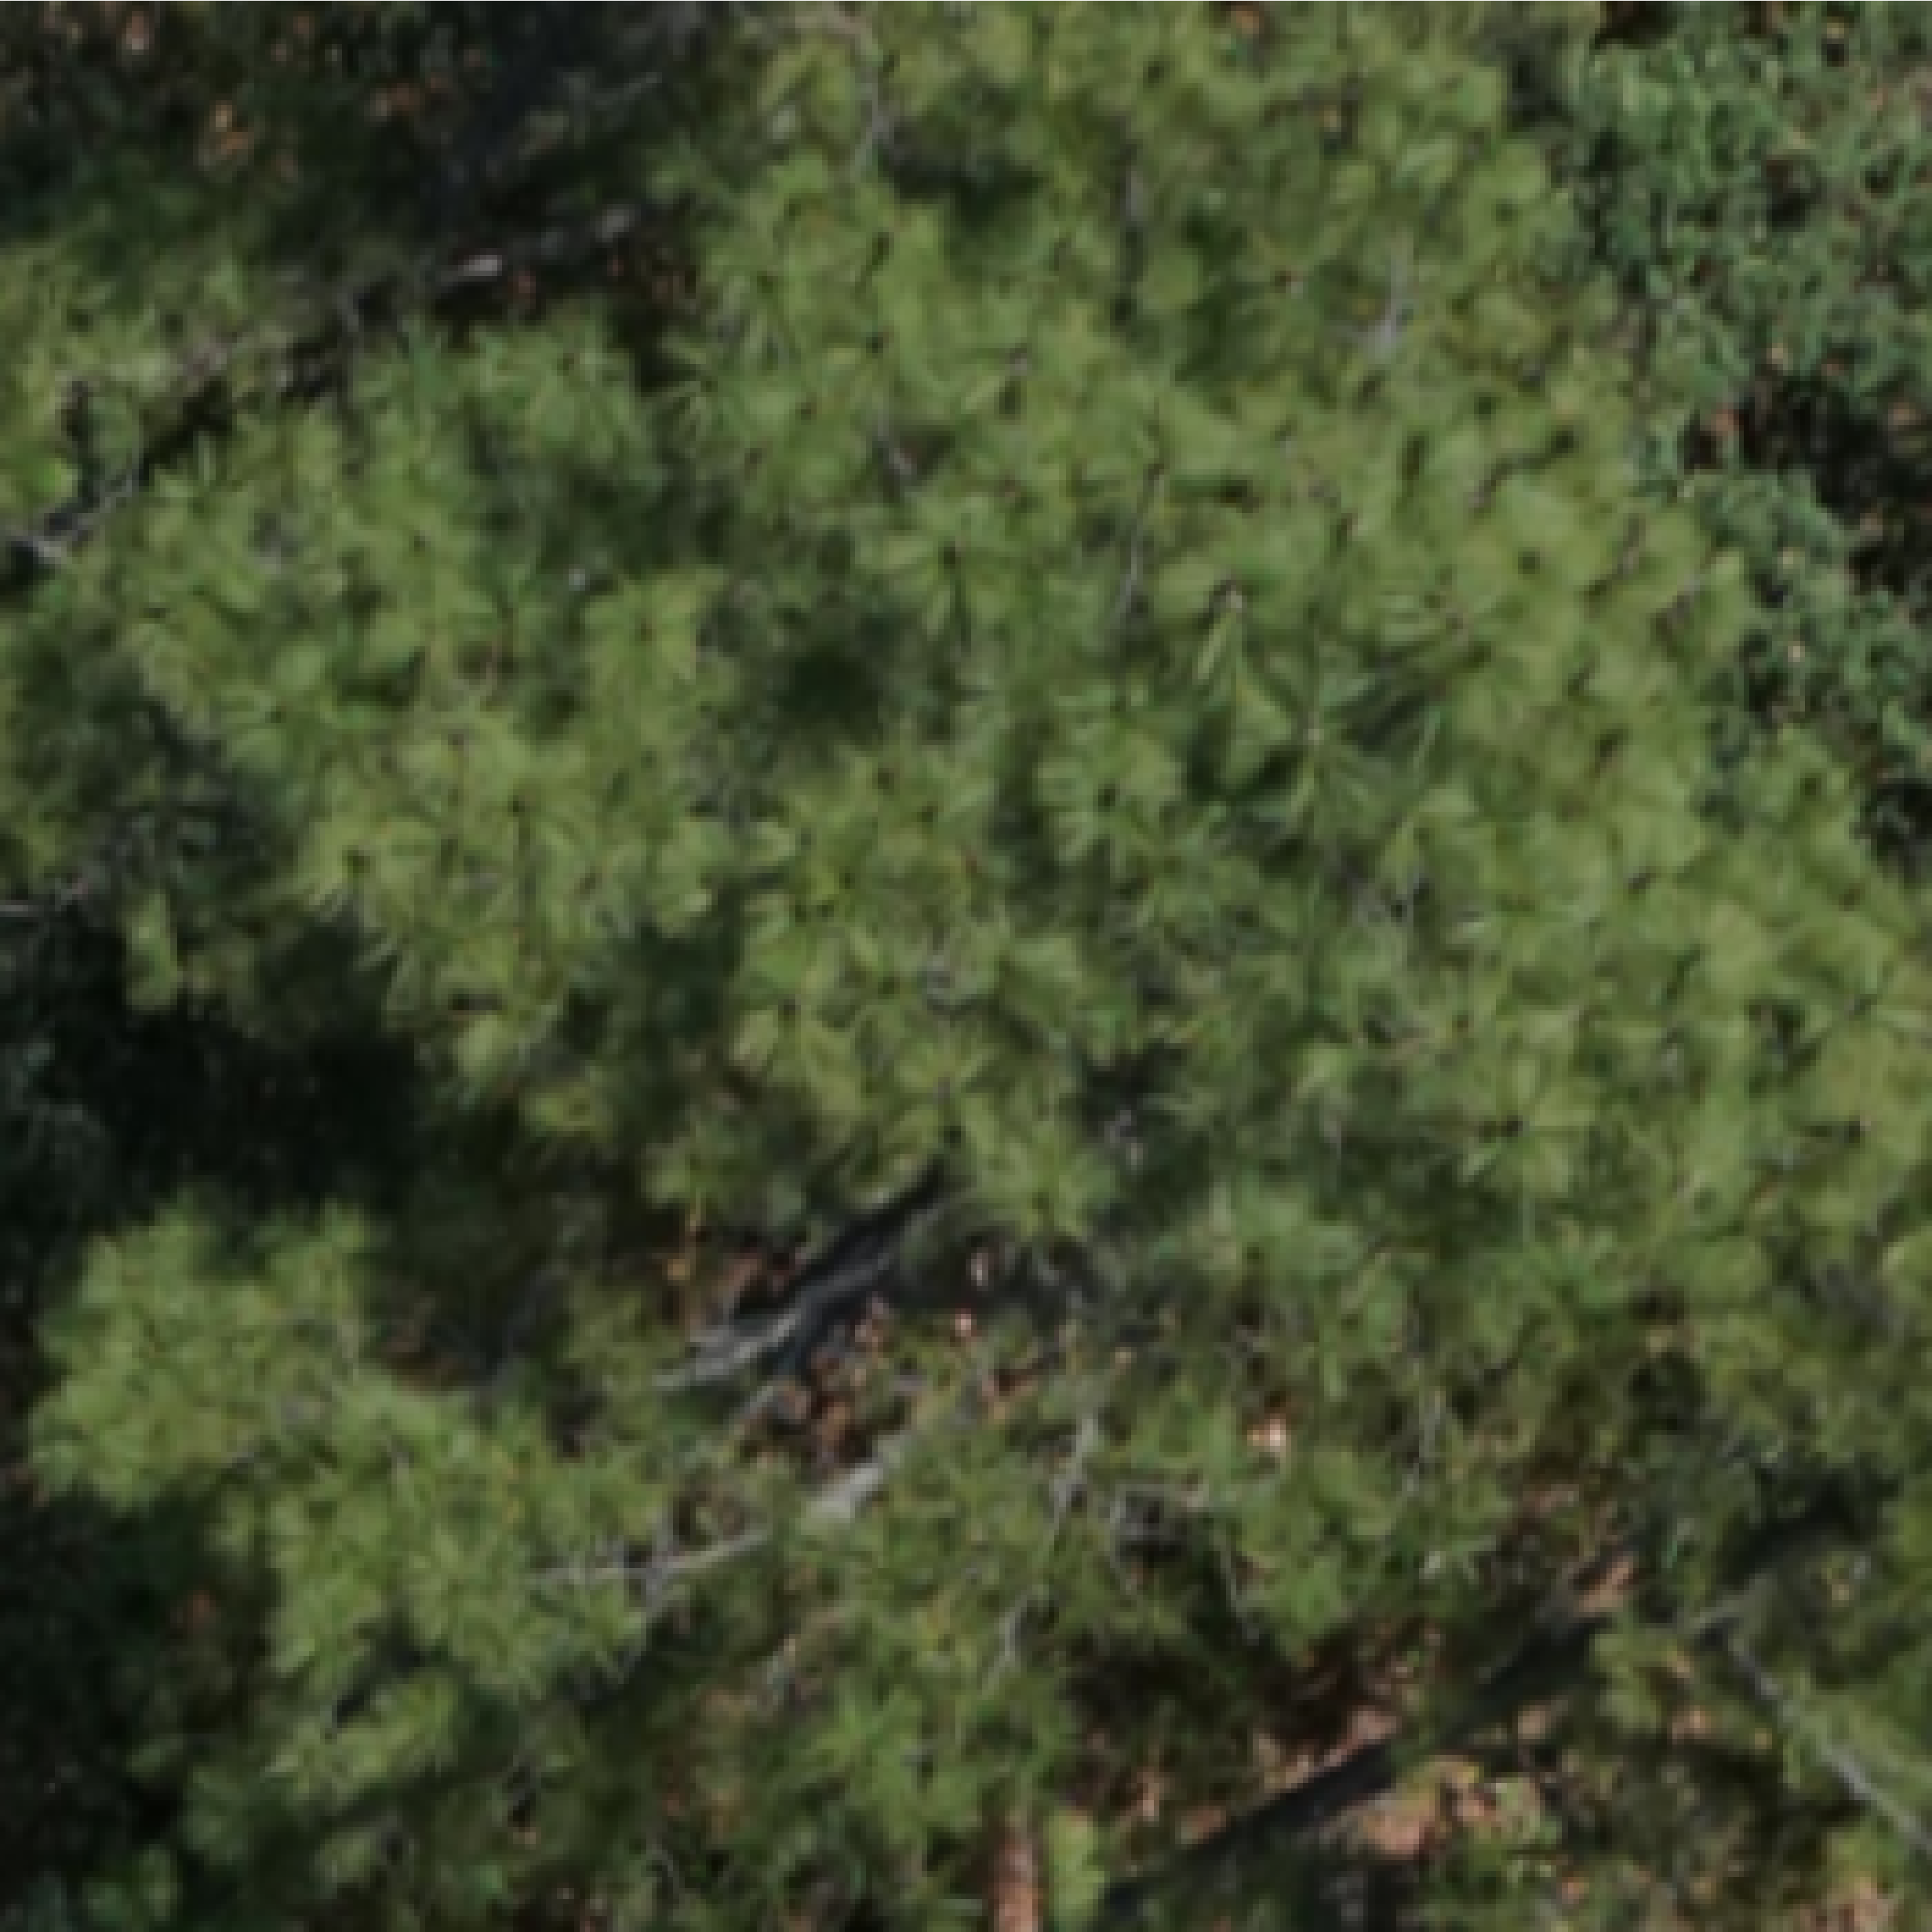
\includegraphics[width=0.3\textwidth]{1_res}} & 
\subfloat[Pino]{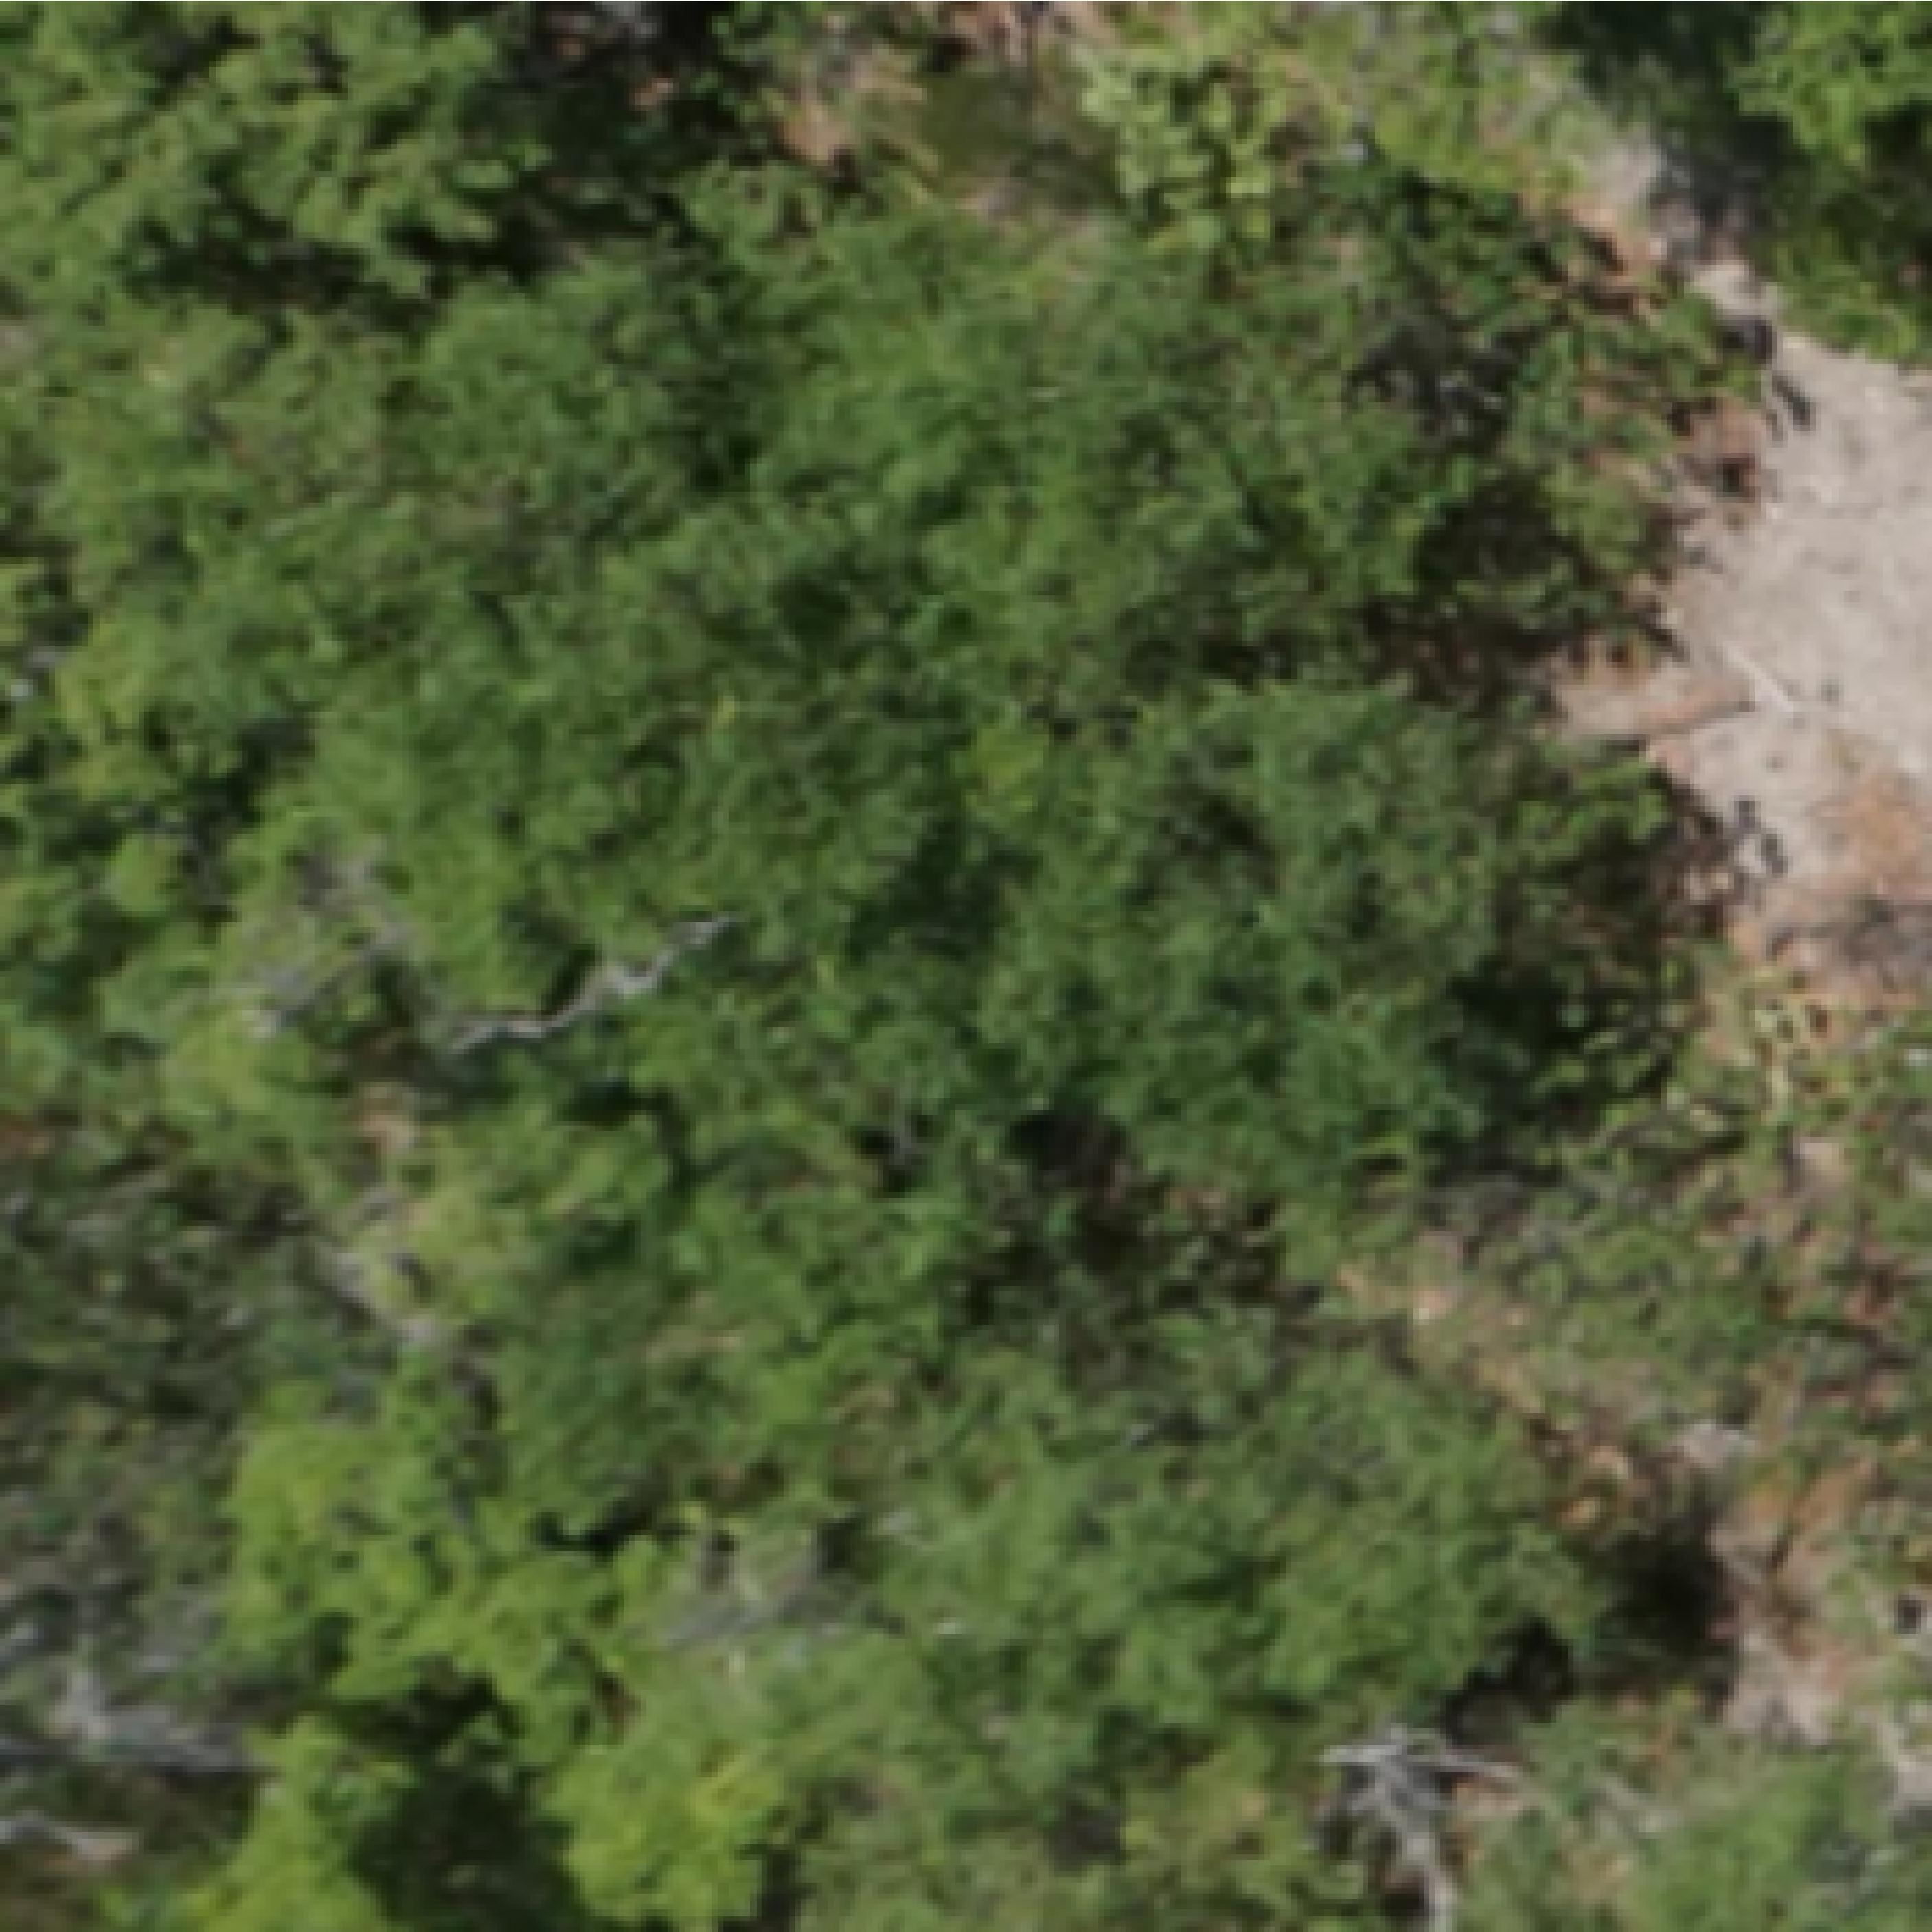
\includegraphics[width=0.3\textwidth]{2_res}} &
\subfloat[Abies]{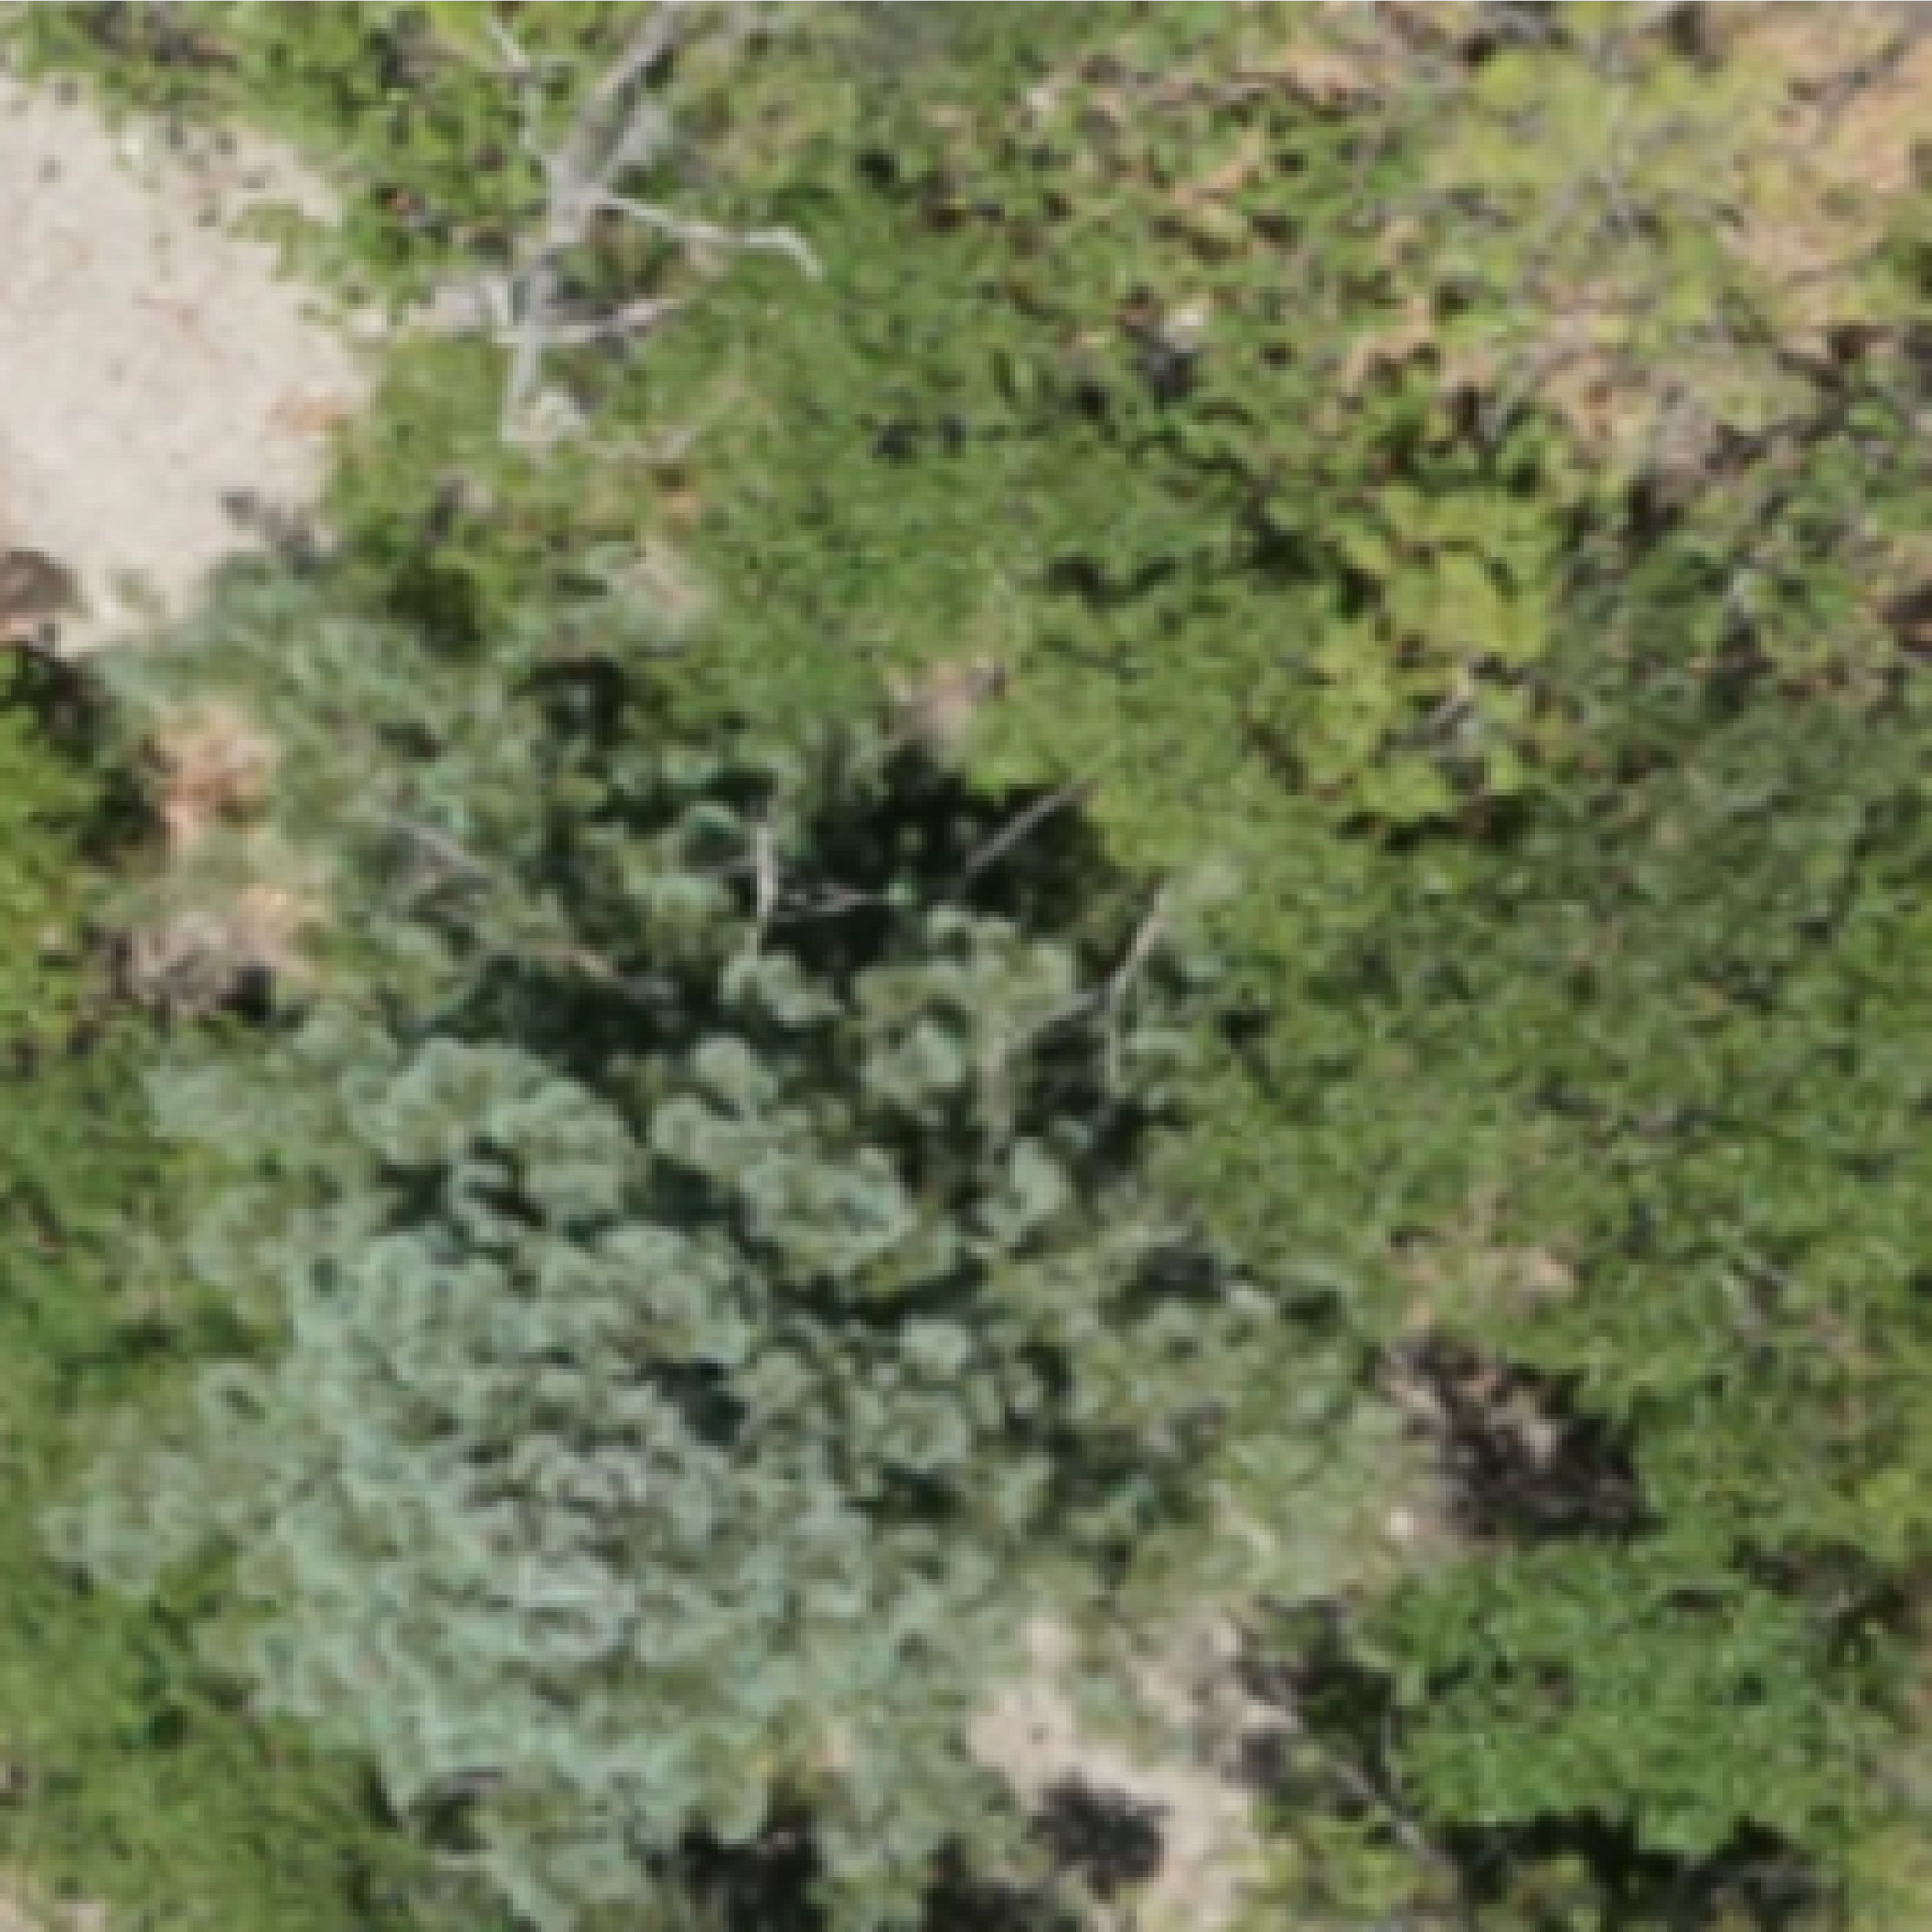
\includegraphics[width=0.3\textwidth]{3_res}}
  \end{tabular}
  \caption[Comparación de texturas.]{Comparación de texturas encontradas.}
  \label{Texturas}
\end{figure}


\subsection{Descriptores de características locales}
Como se menciono al inicio de la sección 2.2, las características locales son necesarias para describir los puntos o regiones de interés en una imagen. 

\begin{description}
\item[Escalamiento:]{Transforma los datos de las características en rangos específicos de cero a uno.}

\item[Normalización:]{Desplaza y re-escala valores para alcanzar un rango entre cero y uno.}

\item[SIFT (Característica de transformación de escala invariante)]{Extrae la información y adecua en comparaciones.}

\item[SURF (Característica de acelerado robusto)]{Toma un vecino al rededor del punto seleccionado en la imagen y es dividido en sub-regiones para cada sub-región.}

\item[BRIEF (Característica de diferencias en forma de cadena binaria)]{Se enfoca en la orientación y menor numero de diferencias a su alrededor.}

\item[ORB (BRIEF rotada y orientada rápida)]{Determina estos puntos clave de una imágen.}
\end{description}

\subsection{Uso de descriptores}
Existen varias formas de utilizar los descriptores pero hay dos maneras de mezclar las características de vectores.

\paragraph{Para las características globales de vector, sólo se concatena cada característica del vector para formar a una característica global del vector simple. Este enfoque se utiliza en el desarrollo de este algoritmo} 

\paragraph{Para las características locales del vector también puede hacerse una combinación de las características locales y globales del vector, es necesario algo llamado \emph{modelo de la bolsa de palabras} (BOVW). Este enfoque se utiliza normalmente en constructores de vocabularios, agrupamiento de $K$-medias, etc} 

\section{Trabajos relacionados}
Existen algunos trabajos que no están completamente relacionados con el objetivo de identificar especies arbóreas, pero si existen investigaciones que toman como objetivo el analizar zonas forestales.

\citet{rf14} menciona como hacen uso de combinar datos para realizar inventarios forestales por medio de sistemas digitales aéreos de fotogrametría y escáneres láser. Con estas tecnologías, hacen una búsqueda buscando los tipos predominantes en una zona y con ayuda del \emph{análisis de imágenes basado en objetos} se pudo admitir la delineación automática de árboles, la clasificación de especies arbóreas y la definición de atributos estructurales a nivel de árbol. 
\newline
\break

\citet{rf1}  utilizan una gran cantidad de entradas para definir manualmente la especie, no obstante, la principal diferencia es que este trabajo no realiza un inventario forestal por medio de visión computacional sino por técnicas tradicionales.
 
\citet{rf2} tienen como meta evaluar artículos para actualizar los inventarios de árboles en un área metropolitana. En este no se trata con inteligencia artificial como tal, pero si hacen uso de tecnologías de detección como sensores remotos que permitan evaluar correctamente y obtengan la información concreta de las zonas donde habitan  árboles.

\citet{rf3} tienen como objetivo detectar objetos además de hacer uso del umbral adaptativo, el cual es muy utilizado en la visión computacional. %El problema a solucionar en concreto como parte de este trabajo es, resolver los métodos de umbralización.

\citet{rf9} hace simulaciones para la gestión de modelos forestales que podría ser requeridos para la toma de decisiones en un sector forestal. En este artículo se hacen validaciones usando modelos generados por información de un bosque privado y un bosque estatal de Illinois, EE.UU.

\citet{rf10} hacen uso de técnicas de inteligencia artificial para la identificación  de especies forestales haciendo uso de multidatos espectrales tomando como punto de partida, los vecinos más cercanos (KNN) para procesar eficientemente la información recolectada y segmentar por clusters el ambiente sobre el que se trabajó.

\begin{table}[h!]
\centering
\caption{Comparación de trabajos frente al desarrollado, donde \checkmark indica que cumple con esta característica y  $\times$ no cumple con esta característica.}
\vspace{0.5cm}
\begin{adjustbox}{width=0.5\textwidth}
\begin{tabular}{|l|c|c|c|}
\hline
Trabajo & \rotatebox[origin=c]{90}{Inventarios forestales}& \rotatebox[origin=c]{90}{Visión computacional} & \rotatebox[origin=c]{90}{ Detección de objetos}\\
	\hline
    \citet{rf1} & \checkmark & $\times$ & \checkmark\\
    \hline
    \citet{rf2}&  \checkmark  &  $\times$ & $\times$ \\
    \hline
    \citet{rf3}& $\times$ & \checkmark & \checkmark\\
    \hline
    \citet{rf9}& \checkmark & \checkmark & \checkmark\\
	\hline    
    \citet{rf10}& $\times$ & \checkmark & \checkmark\\
	\hline    
    \citet{rf11}& $\times$ & \checkmark & \checkmark\\
	\hline    
    \citet{rf12}& \checkmark  & $\times$ & $\times$\\
	\hline    
    \citet{rf13}& \checkmark & $\times$ & $\times$\\
	\hline    
    \citet{rf14}&  $\times$ & \checkmark & $\times$\\
	\hline    
    \citet{rf15}& \checkmark & \checkmark & $\times$\\
	\hline    
    El presente trabajo & \checkmark & \checkmark & \checkmark\\
    \hline
\end{tabular}
\end{adjustbox}
\label{tab:Comparación de trabajos frente al desarrollado}
\end{table}
\section{Solución propuesta}

\section{Evaluación}

\section{Conclusiones}

\section{Referencias bibliográficas}

\bibliography{mybibfile}

\end{document}